% Created 2022-08-19 vie 13:36
% Intended LaTeX compiler: pdflatex
\documentclass[aspectratio=169, usenames,svgnames,dvipsnames]{beamer}
\usepackage[utf8]{inputenc}
\usepackage[T1]{fontenc}
\usepackage{graphicx}
\usepackage{grffile}
\usepackage{longtable}
\usepackage{wrapfig}
\usepackage{rotating}
\usepackage[normalem]{ulem}
\usepackage{amsmath}
\usepackage{textcomp}
\usepackage{amssymb}
\usepackage{capt-of}
\usepackage{hyperref}
\usepackage{color}
\usepackage{listings}
\usepackage{mathpazo}
\usepackage{gensymb}
\usepackage{amsmath}
\usepackage{diffcoeff}
\usepackage{steinmetz}
\usepackage{mathtools}
\bibliographystyle{plain}
\usepackage{siunitx}
\sisetup{output-decimal-marker={,}}
\DeclareSIUnit{\watthour}{Wh}
\hypersetup{colorlinks=true, linkcolor=Blue, urlcolor=Blue}
\renewcommand{\thefootnote}{\fnsymbol{footnote}}
\newcommand{\laplace}[1]{\mathbf{#1}(\mathbf{s})}
\newcommand{\slp}{\mathbf{s}}
\newcommand{\fasor}[1]{\mathbf{#1}(\omega)}
\newcommand{\atan}{\mathrm{atan}}
\parskip=5pt
\usetheme{Boadilla}
\usecolortheme{rose}
\usefonttheme{serif}
\author{Oscar Perpiñán Lamigueiro}
\date{}
\title{Corriente alterna sinusoidal}
\subtitle{Teoría de Circuitos}
\setbeamercolor{alerted text}{fg=blue!50!black} \setbeamerfont{alerted text}{series=\bfseries}
\AtBeginSubsection[]{\begin{frame}[plain]\tableofcontents[currentsubsection,sectionstyle=show/shaded,subsectionstyle=show/shaded/hide]\end{frame}}
\AtBeginSection[]{\begin{frame}[plain]\tableofcontents[currentsection,hideallsubsections]\end{frame}}
\beamertemplatenavigationsymbolsempty
\setbeamertemplate{footline}[frame number]
\setbeamertemplate{itemize items}[triangle]
\setbeamertemplate{enumerate items}[circle]
\setbeamertemplate{section in toc}[circle]
\setbeamertemplate{subsection in toc}[circle]
\hypersetup{
 pdfauthor={Oscar Perpiñán Lamigueiro},
 pdftitle={Corriente alterna sinusoidal},
 pdfkeywords={},
 pdfsubject={},
 pdfcreator={Emacs 27.1 (Org mode 9.4.6)}, 
 pdflang={Spanish}}
\begin{document}

\maketitle

\section{Formas de Onda}
\label{sec:orgf89fccf}

\begin{frame}[label={sec:org89598b2}]{Forma de Onda}
\begin{itemize}
\item La salida de los generadores (de tensión o de corriente) son funciones que pueden variar con el tiempo.
\item La dependencia funcional \(u = u(t)\) o \(i = i(t)\) se denomina forma de onda.
\end{itemize}
\end{frame}
\begin{frame}[label={sec:org30cbb1b}]{Clasificación}
\begin{block}{Signo de la magnitud}
\begin{itemize}
\item Unidireccionales
\begin{itemize}
\item Signo constante
\item El valor puede ser constante (corriente continua) o variable.
\end{itemize}
\item Bidireccionales
\begin{itemize}
\item Signo variable con el tiempo.
\end{itemize}
\end{itemize}
\end{block}
\begin{block}{Repetición del valor de la magnitud}
\begin{itemize}
\item Periódicas

El valor de la magnitud se repite de forma regular.

\item No periódicas

El valor de la magnitud varía de forma arbitraria con el tiempo.
\end{itemize}
\end{block}
\end{frame}

\begin{frame}[label={sec:orgb882861}]{Valores que definen una onda periódica}
\begin{block}{Período y frecuencia}
\begin{itemize}
\item Período (\(T\)): tiempo que tarda en repetirse la función.
\item Frecuencia (\(f\)): número de repeticiones por unidad de tiempo.
\item \(f = \frac{1}{T}\)
\end{itemize}
\end{block}
\begin{block}{Valor medio}
\[
U_m=\frac{1}{T}\int_{0}^{T}u(t)\, dt \qquad \qquad%
I_m=\frac{1}{T}\int_{0}^{T}i(t)\, dt
\]
\end{block}

\begin{block}{Valor eficaz}
\[
U = \sqrt{\frac{1}{T}\cdot\int_{0}^{T}u^{2}(t)\, dt} \qquad \qquad%
I = \sqrt{\frac{1}{T}\cdot\int_{0}^{T}i^{2}(t)\, dt}
\]
\end{block}
\end{frame}

\begin{frame}[label={sec:org8fbebab}]{Valores que definen una onda periódica}
\begin{itemize}
\item Valores de pico

\[
Y_{max} = \max(y(t)) \qquad Y_{min} = \min(y(t))
\]

\item Amplitud o valor pico a pico
\end{itemize}

\[
 |Y_{max} - Y_{min}|
\]

\begin{itemize}
\item Factor de amplitud
\end{itemize}

\[FA = \frac{Y_{max}}{Y}\]

\begin{itemize}
\item Factor de forma
\end{itemize}

\[FF = \frac{Y}{Y_{m}}\]
\end{frame}


\begin{frame}[label={sec:org213d147}]{Formas de Onda Periódicas}
\framesubtitle{Tren de Pulsos Bidireccional}
\begin{center}
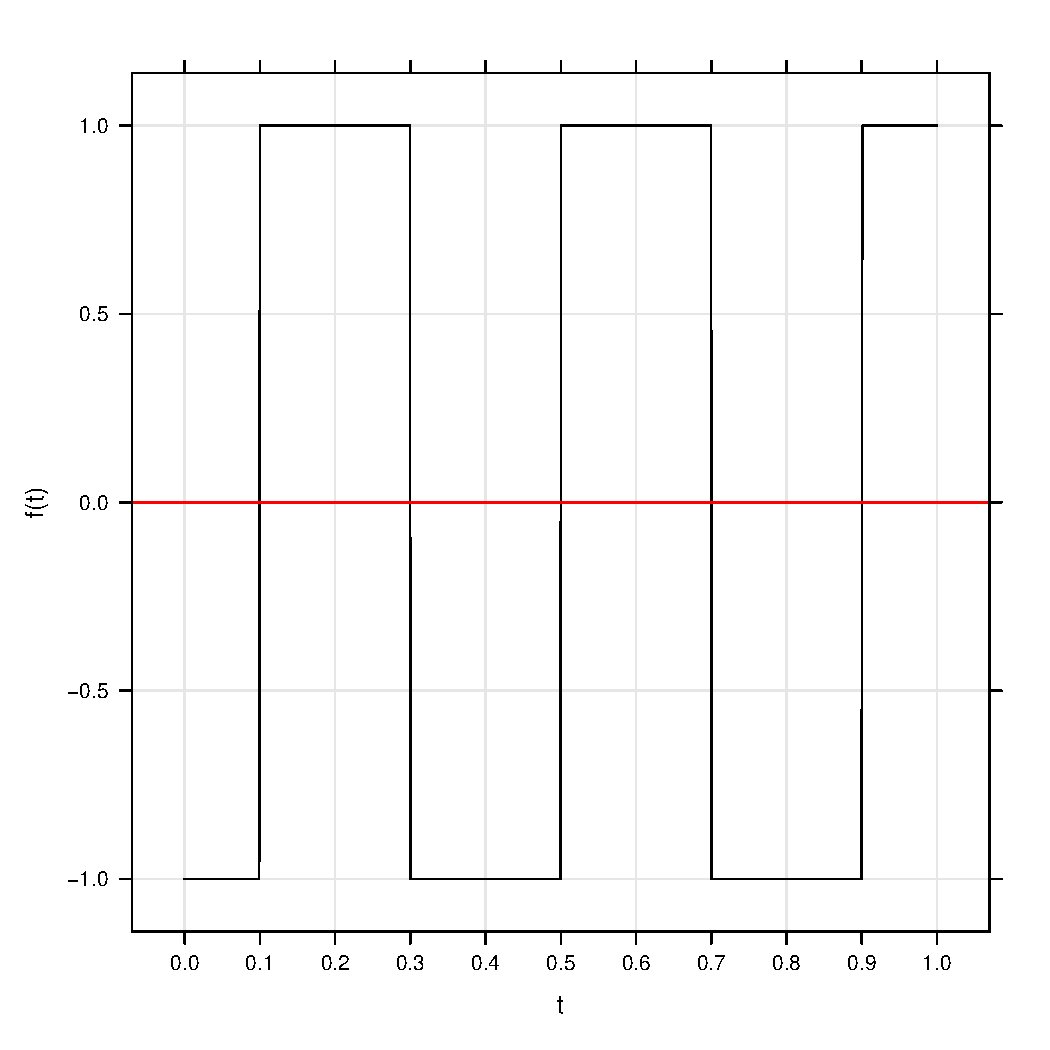
\includegraphics[height=0.9\textheight]{../figs/cuadrada_periodica.pdf}
\end{center}
\end{frame}

\begin{frame}[label={sec:org6399c74}]{Formas de Onda Periódicas}
\framesubtitle{Tren de Pulsos Unidireccional}
\begin{center}
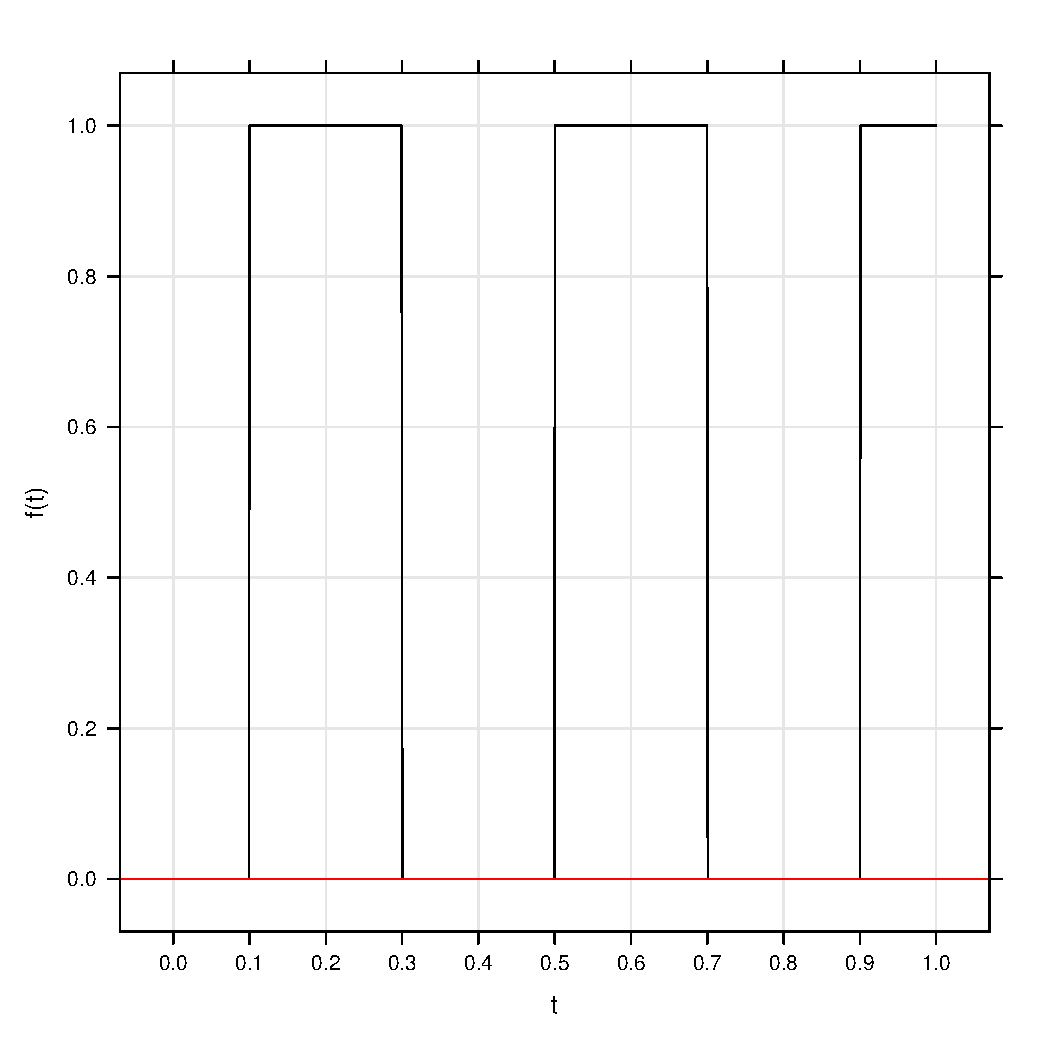
\includegraphics[height=0.9\textheight]{../figs/cuadrada0_periodica.pdf}
\end{center}
\end{frame}

\begin{frame}[label={sec:orge027c12}]{Formas de Onda Periódicas}
\framesubtitle{Onda Triangular Bidireccional}
\begin{center}
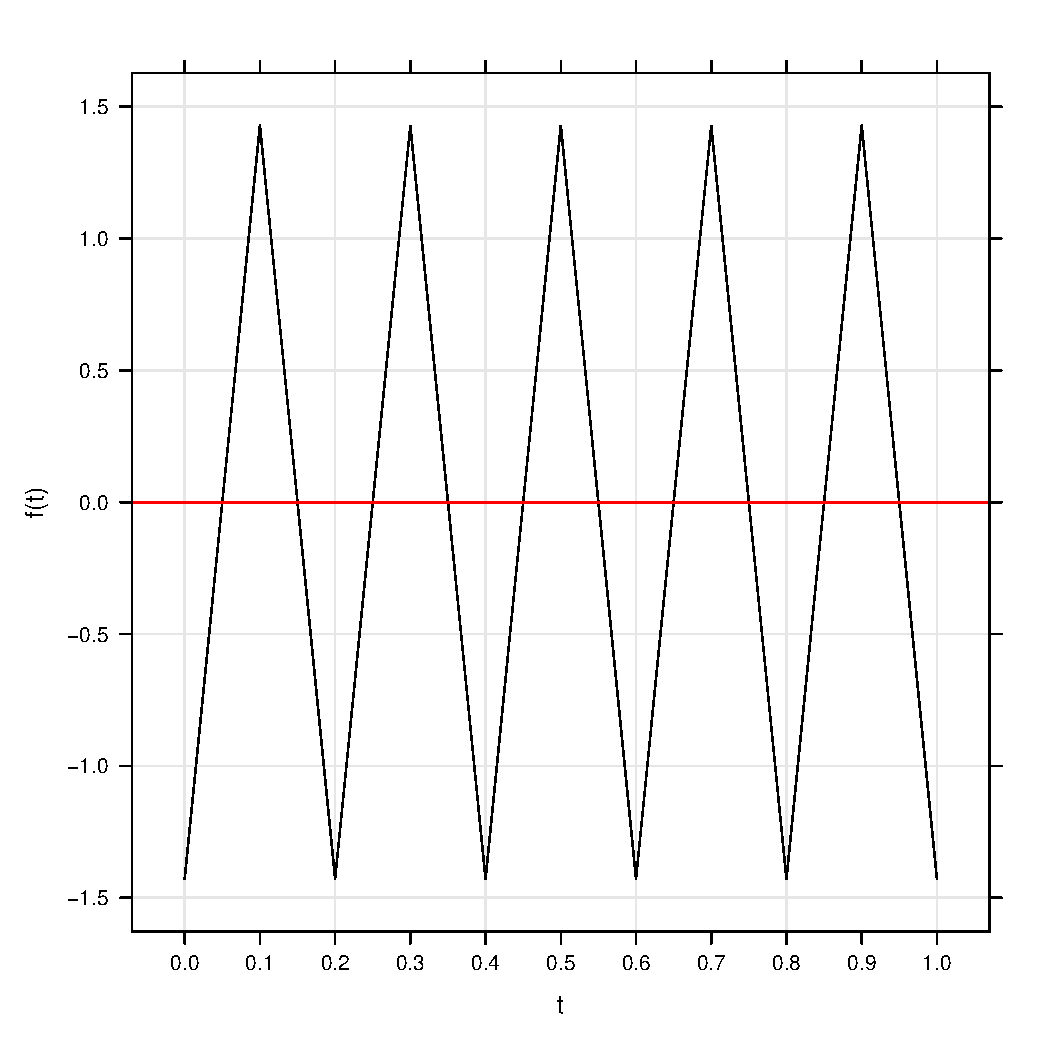
\includegraphics[height=0.9\textheight]{../figs/triangular_periodica.pdf}
\end{center}
\end{frame}
\begin{frame}[label={sec:org027bb61}]{Formas de Onda Periódicas}
\framesubtitle{Onda Triangular Unidireccional}
\begin{center}
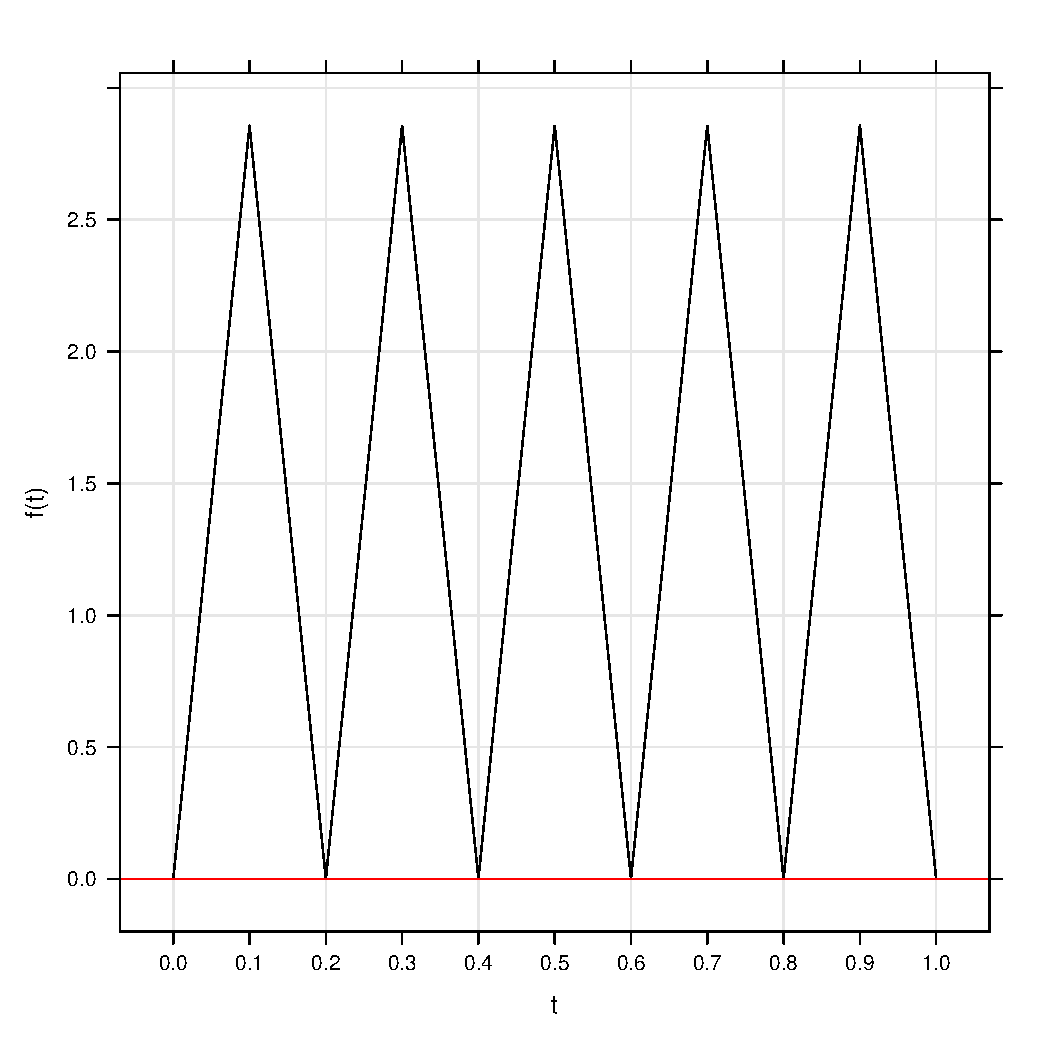
\includegraphics[height=0.9\textheight]{../figs/triangular0_periodica.pdf}
\end{center}
\end{frame}

\begin{frame}[label={sec:org9b69f99}]{Formas de Onda Periódicas}
\framesubtitle{Onda sinusoidal}

\begin{center}
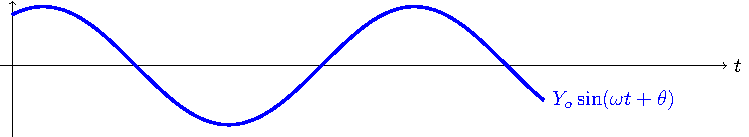
\includegraphics[width=.9\linewidth]{../figs/sin.pdf}
\end{center}
\end{frame}

\section{Onda Sinusoidal}
\label{sec:org7bcf962}

\begin{frame}[label={sec:org7a5e661}]{Definición}
\begin{center}
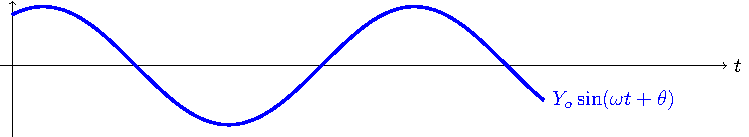
\includegraphics[width=.9\linewidth]{../figs/sin.pdf}
\end{center}


\[
y(t)=Y_{o}\cdot\sin(\omega\cdot t+\theta)
\]

\begin{itemize}
\item \(Y_{o}\) valor máximo de la onda.

\item T: periodo de la onda (segundos)

\item \(\omega=\frac{2\cdot\pi}{T}\): pulsación (radianes/segundo)

\item \(f=\frac{\omega}{2\cdot\pi}=\frac{1}{T}\): frecuencia (Hz)

\item \(\theta\): fase (radianes o grados)
\end{itemize}
\end{frame}


\begin{frame}[label={sec:org0d32d6c}]{Fase}
\begin{center}
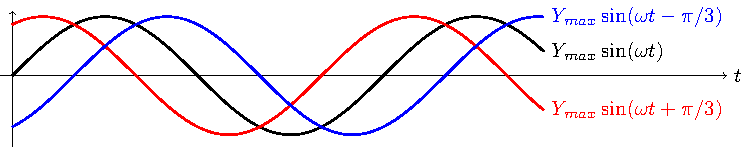
\includegraphics[width=.9\linewidth]{../figs/desfase.pdf}
\end{center}


\[
y(t)=Y_{o}\cdot\sin(\omega\cdot t+\theta)
\]

\begin{itemize}
\item \(\theta\): fase (radianes o grados)

\begin{itemize}
\item Es el argumento de la onda para t=0

\item Tomando una onda como referencia, si la fase es 0º, se dice que
están en fase con la onda de referencia.

\item Si la fase es positiva, se dice que la onda adelanta
respecto a la referencia.
\end{itemize}
\end{itemize}
\end{frame}


\begin{frame}[label={sec:org0683624}]{Señales en Cuadratura}
\begin{center}
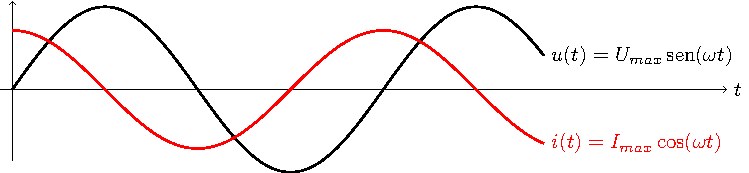
\includegraphics[width=.9\linewidth]{../figs/cuadratura.pdf}
\end{center}

\begin{itemize}
\item Cuando el desfase entre dos señales es de 90º (\(\theta_I - \theta_U = \pi/2\)), se dice que están en cuadratura.
\item El paso por cero de una señal coincide con el paso por el máximo/mínimo de la otra señal.
\end{itemize}
\end{frame}


\begin{frame}[label={sec:orgeedd2ff}]{Valor medio y valor eficaz}
\begin{block}{Valor medio}
\[
Y_m=\frac{1}{T}\int_{0}^{T}y(t)\, dt
\]

\[
Y_m=\frac{1}{T}\int_{0}^{T}Y_{o}\cdot\sin(\omega \cdot t+\theta)\, dt=0
\]
\end{block}
\begin{block}{Valor eficaz}
\[
Y = \sqrt{\frac{1}{T}\cdot\int_{0}^{T}y^{2}(t)\, dt}
\]

\[
Y=\sqrt{\frac{1}{T}\cdot\int_{0}^{T}\left(Y_{o}\cdot\sin(\omega\cdot t+\theta)\right)^{2}dt}=\boxed{\frac{Y_{o}}{\sqrt{2}}}
\]
\end{block}
\end{frame}
\section{Cálculo Fasorial}
\label{sec:orgc80d484}

\begin{frame}[label={sec:org82a3048}]{Representación fasorial}
\begin{itemize}
\item Un fasor es un \alert{número complejo} que representa una señal sinusoidal para simplificar cálculos.
\item El \alert{módulo} del fasor es el \alert{valor eficaz}. El \alert{argumento} es la \alert{fase}.
\item Descartamos pulsación: No se puede emplear cuando hay frecuencias diferentes en un mismo circuito.
\end{itemize}

\begin{columns}
\begin{column}{0.5\columnwidth}
\begin{align*}
\overline{Y} &= Y\cdot e^{j\theta}\\
\overline{Y} &= Y\phase{\theta}\\
\overline{Y} &= Y\cdot(\cos(\theta)+\mathrm{j}\cdot\sin(\theta))
\end{align*}
\end{column}

\begin{column}{0.5\columnwidth}
\begin{center}
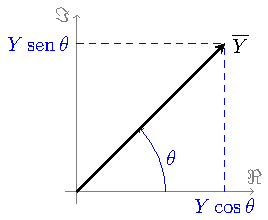
\includegraphics[height=0.45\textheight]{../figs/fasor.pdf}
\end{center}
\end{column}
\end{columns}
\end{frame}

\begin{frame}[label={sec:orgae2ed95}]{Tensión y corriente en notación fasorial}
\begin{center}
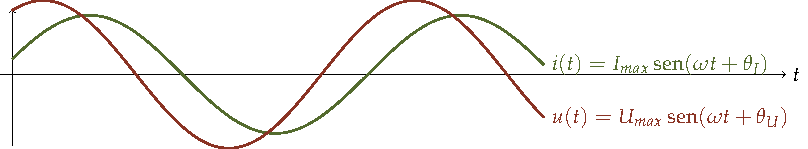
\includegraphics[width=.9\linewidth]{../figs/ondasTensionCorriente.pdf}
\end{center}

\begin{columns}
\begin{column}{0.5\columnwidth}
\begin{align*}
  \overline{U} &= U\phase{\theta_U}\\
  \overline{I} &= I\phase{\theta_I}
\end{align*}
\end{column}

\begin{column}{0.5\columnwidth}
\begin{center}
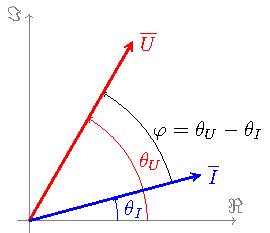
\includegraphics[height=0.5\textheight]{../figs/fasorTensionCorriente.pdf}
\end{center}
\end{column}
\end{columns}
\end{frame}


\begin{frame}[label={sec:org1609ae8}]{Impedancia: relación entre fasores de tensión y corriente}
\begin{columns}
\begin{column}{0.5\columnwidth}
\begin{align*}
  \overline{U} &= \overline{Z} \cdot \overline{I}\\                 
  \overline{Z} &= \frac{\overline{U}}{\overline{I}}
\end{align*}
\end{column}

\begin{column}{0.5\columnwidth}
\begin{center}
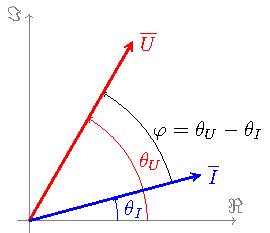
\includegraphics[height=0.5\textheight]{../figs/fasorTensionCorriente.pdf}
\end{center}
\end{column}
\end{columns}

\[
\boxed{\overline{Z} = \frac{U}{I}\phase{\theta_U - \theta_I} \Rightarrow 
    \begin{cases}
      Z = \frac{U}{I}\\
      \theta = \theta_U - \theta_I
    \end{cases}}
\]
\end{frame}



\begin{frame}[label={sec:org3abcbc7}]{Impedancia Genérica}
\[
\overline{Z} = R + j X
\]

\begin{center}
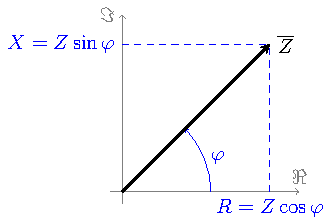
\includegraphics[height=0.75\textheight]{../figs/fasorImpedancia.pdf}
\end{center}
\end{frame}

\begin{frame}[label={sec:orgfbd9cbb}]{Circuito Resistivo}
Un circuito resistivo no desfasa (\alert{tensión y corriente en fase}).

\begin{center}
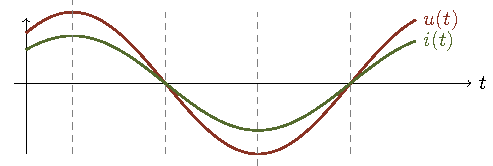
\includegraphics[height=0.4\textheight]{../figs/resistivo.pdf}
\end{center}

\[
    i(t) = I_o \cdot \sin(\omega t + \theta_I)
\]
\begin{align*}
  u(t) &= R \cdot i(t)=\\
       &= {\color{blue}R I_o} \cdot \sin(\omega t + {\color{red!80}\theta_I + 0}) =\\
       &= {\color{blue}U_o} \cdot \sin(\omega t + {\color{red!80} \theta_I + 0})\\
\end{align*}
\end{frame}

\begin{frame}[label={sec:org6e0c09f}]{Circuito Resistivo}
Un circuito resistivo no desfasa (\alert{tensión y corriente en fase}).
\begin{center}
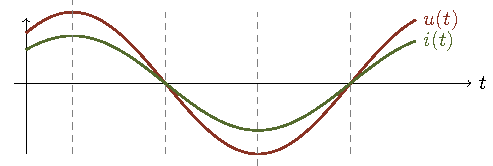
\includegraphics[height=0.3\textheight]{../figs/resistivo.pdf}
\end{center}

\begin{columns}
\begin{column}{0.3\columnwidth}
\begin{align*}
  Z &= \frac{U}{I} = R\\
  \theta &= \theta_U - \theta_I = 0\\
  \Aboxed{\overline{Z}_R &= R \phase{0}}
\end{align*}
\end{column}

\begin{column}{0.35\columnwidth}
\begin{center}
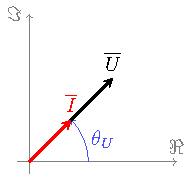
\includegraphics[height=0.35\textheight]{../figs/fasorResistencia_VI.pdf}
\end{center}
\end{column}


\begin{column}{0.35\columnwidth}
\begin{center}
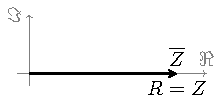
\includegraphics[height=0.25\textheight]{../figs/fasorResistencia.pdf}
\end{center}
\end{column}
\end{columns}
\end{frame}



\begin{frame}[label={sec:orge0cffd1}]{Circuito Inductivo puro}
Un circuito inductivo puro genera \alert{señales en cuadratura} y \alert{retrasa la corriente}.
\begin{center}
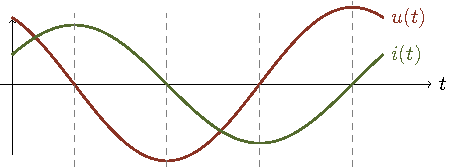
\includegraphics[height=0.3\textheight]{../figs/inductivoPuro.pdf}
\end{center}

\[
    i(t) = I_o \cdot \sin(\omega t + \theta_I)
\]
\begin{align*}
  u(t) &= L \cdot \frac{d i(t)}{dt} =\\
       &= {\color{blue}{\omega L I_o}} \cdot \sin(\omega t + {\color{red!80}{\theta_I +\pi/2}}) =\\
       &= {\color{blue}{U_o}} \cdot \sin(\omega t +  {\color{red!80}{\theta_I +\pi/2}})\\
\end{align*}
\end{frame}


\begin{frame}[label={sec:org1699bc9}]{Circuito Inductivo puro}
Un circuito inductivo puro genera \alert{señales en cuadratura} y \alert{retrasa la corriente}.

\begin{center}
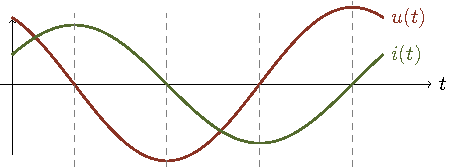
\includegraphics[height=0.3\textheight]{../figs/inductivoPuro.pdf}
\end{center}

\begin{columns}
\begin{column}{0.3\columnwidth}
\begin{align*}
  Z &= \frac{U}{I} = \omega L\\
  \theta &= \theta_U - \theta_I = \pi/2\\
  \Aboxed{\overline{Z}_L &= j\omega L = \omega L \phase{\ang{90}}}
\end{align*}
\end{column}


\begin{column}{0.4\columnwidth}
\begin{center}
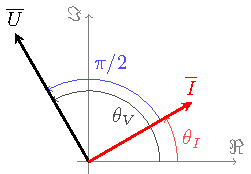
\includegraphics[height=0.4\textheight]{../figs/fasorInductancia_VI.pdf}
\end{center}
\end{column}


\begin{column}{0.3\columnwidth}
\begin{center}
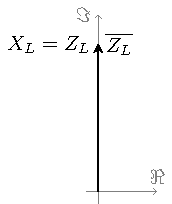
\includegraphics[height=0.4\textheight]{../figs/fasorInductancia.pdf}
\end{center}
\end{column}
\end{columns}
\end{frame}


\begin{frame}[label={sec:orgcb3bc78}]{Circuito Capacitivo puro}
Un circuito capacitivo puro genera \alert{señales en cuadratura} y \alert{adelanta la corriente}.

\begin{center}
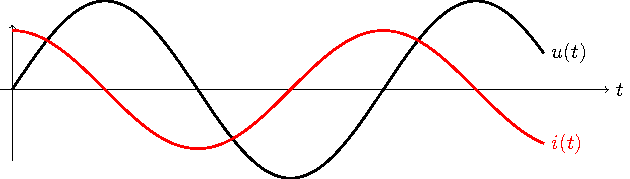
\includegraphics[height=0.3\textheight]{../figs/capacitivoPuro.pdf}
\end{center}

\[
    i(t) = I_o \cdot \sin(\omega t + \theta_I)
\]
\begin{align*}
  u(t) &= 1/C \cdot \int_{-\infty}^ t i(\tau)d\tau =\\
       &= {\color{blue}{\frac{1}{\omega C} I_o}} \cdot \sin(\omega t + {\color{red!80}{\theta_I -\pi/2}}) =\\
       &= {\color{blue}{U_o}} \cdot \sin(\omega t + {\color{red!80}{\theta_I -\pi/2}})\\
\end{align*}
\end{frame}


\begin{frame}[label={sec:orgcc24166}]{Circuito Capacitivo puro}
Un circuito capacitivo puro genera \alert{señales en cuadratura} y \alert{adelanta la corriente}.

\begin{center}
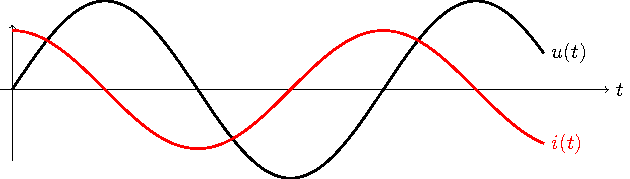
\includegraphics[height=0.3\textheight]{../figs/capacitivoPuro.pdf}
\end{center}

\begin{columns}
\begin{column}{0.3\columnwidth}
\begin{align*}
  Z &= \frac{U}{I} = \frac{1}{\omega C}\\
  \theta &= \theta_U - \theta_I = - \pi/2\\
  \Aboxed{\overline{Z}_C &= \frac{1}{j\omega C} = \frac{1}{\omega C}\phase{\ang{-90}}}
\end{align*}
\end{column}


\begin{column}{0.4\columnwidth}
\begin{center}
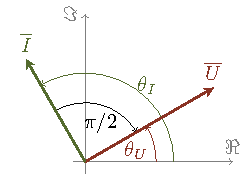
\includegraphics[height=0.4\textheight]{../figs/fasorCondensador_VI.pdf}
\end{center}
\end{column}


\begin{column}{0.3\columnwidth}
\begin{center}
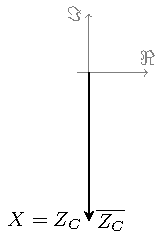
\includegraphics[height=0.4\textheight]{../figs/fasorCondensador.pdf}
\end{center}
\end{column}
\end{columns}
\end{frame}

\begin{frame}[label={sec:org895a008}]{Resumen}
\[
  \begin{array}{lccc}
    \text{Elemento} & \text{Impedancia} & \text{Módulo} & \text{Ángulo}\\
    \hline\\
    \text{Resistencia} & R & R & 0\\
    \text{Bobina} & j \omega L & \omega L & \ang{90}\\
     \text{Condensador} & 1/(j \omega C) & 1/(\omega C) & \ang{-90}\\
  \end{array}
\]
\end{frame}
\begin{frame}[label={sec:orgda1e210}]{Circuito RL (inductivo con pérdidas)}
\begin{center}
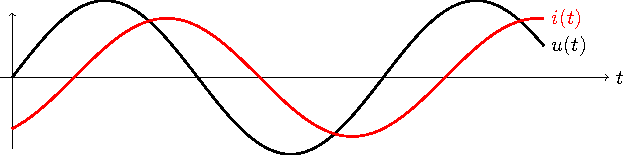
\includegraphics[height=0.25\textheight]{../figs/inductivo.pdf}
\end{center}
\begin{columns}
\begin{column}{0.45\columnwidth}
\begin{center}
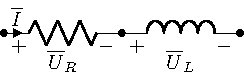
\includegraphics[width=0.8\textwidth]{../figs/RL.pdf}
\end{center}
\end{column}


\begin{column}{0.55\columnwidth}
\begin{center}
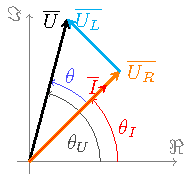
\includegraphics[height=0.5\textheight]{../figs/fasorInductanciaReal_VI.pdf}
\end{center}
\end{column}
\end{columns}
\end{frame}

\begin{frame}[label={sec:org98e544d}]{Circuito RL (inductivo con pérdidas)}
\begin{center}
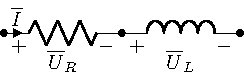
\includegraphics[height=0.2\textheight]{../figs/RL.pdf}
\end{center}

\begin{columns}
\begin{column}{0.45\columnwidth}
\begin{align*}
  \overline{U}_R &= R \overline{I}\\
  \overline{U}_L &= j\omega L \overline{I}
\end{align*}
\end{column}

\begin{column}{0.55\columnwidth}
\begin{align*}
  \overline{U} &= \overline{U}_R + \overline{U}_L =\\
	       &=(R + j\omega L) \overline{I}
\end{align*}
\end{column}
\end{columns}
\end{frame}
\begin{frame}[label={sec:org4aae322}]{Circuito RL (inductivo con pérdidas)}
\begin{center}
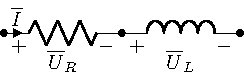
\includegraphics[height=0.2\textheight]{../figs/RL.pdf}
\end{center}

\begin{columns}
\begin{column}{0.45\columnwidth}
\[
\overline{Z} = R + j\omega L \Rightarrow \boxed{\theta > 0}
\]
\[
  |Z| = \sqrt{R^2 + (\omega L)^2}
\]
\[
  \theta = \atan{\frac{\omega L}{R}}
\]
\end{column}

\begin{column}{0.55\columnwidth}
\begin{center}
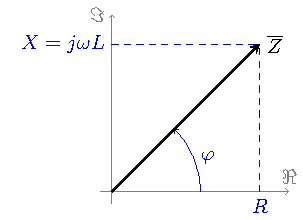
\includegraphics[width=.9\linewidth]{../figs/fasorInductanciaReal.pdf}
\end{center}
\end{column}
\end{columns}
\end{frame}


\begin{frame}[label={sec:org9c97a2d}]{Circuito RC (capacitivo con pérdidas)}
\begin{center}
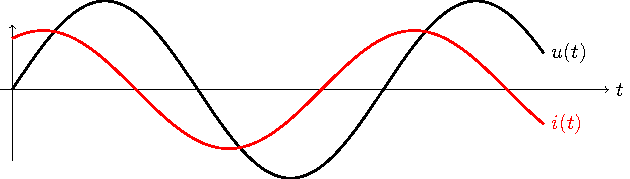
\includegraphics[height=0.25\textheight]{../figs/capacitivo.pdf}
\end{center}


\begin{columns}
\begin{column}{0.45\columnwidth}
\begin{center}
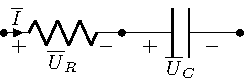
\includegraphics[width=0.8\textwidth]{../figs/RC.pdf}
\end{center}
\end{column}

\begin{column}{0.55\columnwidth}
\begin{center}
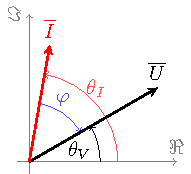
\includegraphics[height=0.45\textheight]{../figs/fasorCondensadorReal_VI.pdf}
\end{center}
\end{column}
\end{columns}
\end{frame}


\begin{frame}[label={sec:org8cc26a3}]{Circuito RC (capacitivo con pérdidas)}
\begin{center}
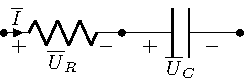
\includegraphics[height=0.2\textheight]{../figs/RC.pdf}
\end{center}

\begin{columns}
\begin{column}{0.45\columnwidth}
\begin{align*}
  \overline{U}_R &= R \overline{I}\\
  \overline{U}_C &= -j \frac{1}{\omega C} \overline{I}
\end{align*}
\end{column}

\begin{column}{0.55\columnwidth}
\begin{align*}
  \overline{U} &= \overline{U}_R + \overline{U}_C =\\
               &= (R - j \frac{1}{\omega C}) \overline{I} 
\end{align*}
\end{column}
\end{columns}
\end{frame}
\begin{frame}[label={sec:org36ebe30}]{Circuito RC (capacitivo con pérdidas)}
\begin{center}
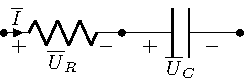
\includegraphics[height=0.2\textheight]{../figs/RC.pdf}
\end{center}

\begin{columns}
\begin{column}{0.45\columnwidth}
\[
\overline{Z} = R - \frac{j}{\omega C} \Rightarrow \boxed{\theta < 0}
\]

\[
  |Z| = \sqrt{R^2 + \frac{1}{(\omega C)^2}}
\]

\[
  \theta = - \atan{\frac{1}{\omega R C}}
\]
\end{column}

\begin{column}{0.55\columnwidth}
\begin{center}
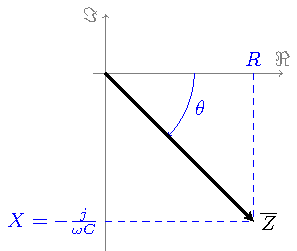
\includegraphics[height=0.45\textheight]{../figs/fasorCondensadorReal.pdf}
\end{center}
\end{column}
\end{columns}
\end{frame}


\begin{frame}[label={sec:org4a10196}]{Circuito RLC serie}
\begin{center}
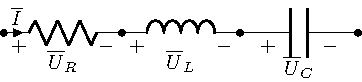
\includegraphics[height=0.2\textheight]{../figs/RLC.pdf}
\end{center}

\begin{columns}
\begin{column}{0.45\columnwidth}
\begin{align*}
  \overline{U}_R &= R \overline{I}\\
  \overline{U}_L &= j\omega L \overline{I}\\
  \overline{U}_C &= -j \frac{1}{\omega C} \overline{I}
\end{align*}
\end{column}

\begin{column}{0.55\columnwidth}
\begin{align*}
  \overline{U} &= \overline{U}_R + \overline{U}_L + \overline{U}_C =\\
               &= \left(R + j(\omega L - \frac{1}{\omega C})\right) \overline{I} 
\end{align*}
\end{column}
\end{columns}
\end{frame}

\begin{frame}[label={sec:org6b07ebf}]{Circuito RLC serie}
\begin{center}
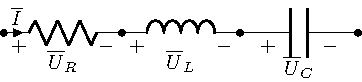
\includegraphics[height=0.2\textheight]{../figs/RLC.pdf}
\end{center}

\begin{columns}
\begin{column}{0.4\columnwidth}
\[
\overline{Z} = R + j(\omega L - \frac{1}{\omega C})
\]
\[
  |Z| = \sqrt{R^2 + (\omega L - \frac{1}{\omega C})^2}
\]
\[
  \theta = \atan{\frac{\omega L - \frac{1}{\omega C}}{R}}
\]
\end{column}

\begin{column}{0.6\columnwidth}
\begin{itemize}
\item \(\theta > 0 \Rightarrow \omega L > \frac{1}{\omega C}\): inductivo
\item \(\theta < 0 \Rightarrow \omega L < \frac{1}{\omega C}\): capacitivo
\item \(\theta = 0 \Rightarrow \omega L = \frac{1}{\omega C}\): resistivo (resonancia)
\end{itemize}
\end{column}
\end{columns}

\[
\boxed{u(t) = Z \cdot I_o \sin(\omega t + \theta_I + \theta)}
\]
\end{frame}

\begin{frame}[label={sec:org5a15c48}]{Circuito RLC paralelo}
\begin{center}
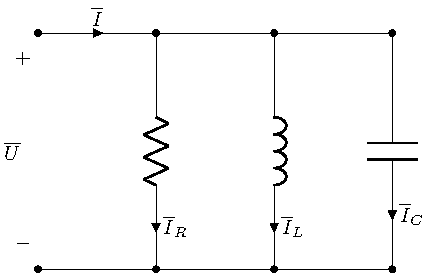
\includegraphics[height=0.45\textheight]{../figs/RLCparalelo.pdf}
\end{center}

\begin{columns}
\begin{column}{0.45\columnwidth}
\begin{align*}
  \overline{I}_R &= 1/R \cdot \overline{U}\\
  \overline{I}_L &= -j \frac{1}{\omega L} \cdot \overline{U}\\
  \overline{I}_C &= j \omega C \cdot \overline{U}
\end{align*}
\end{column}

\begin{column}{0.55\columnwidth}
\begin{align*}
  \overline{I} &= \overline{I}_R + \overline{I}_L + \overline{I}_C =\\
               &= \left(\frac{1}{R} + j(\omega C - \frac{1}{\omega L})\right) \overline{U} 
\end{align*}
\end{column}
\end{columns}
\end{frame}

\begin{frame}[label={sec:org0655c5f}]{Circuito RLC paralelo}
\begin{center}
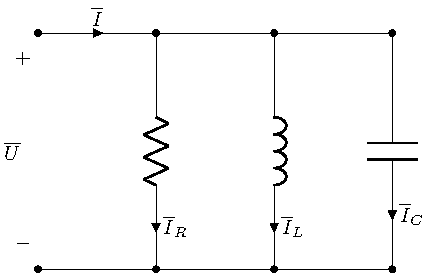
\includegraphics[height=0.45\textheight]{../figs/RLCparalelo.pdf}
\end{center}

\begin{columns}
\begin{column}{0.4\columnwidth}
\[
\overline{Y} = \frac{\overline{I}}{\overline{U}} = 1/R + j(\omega C - \frac{1}{\omega L})
\]
\[
  |Y| = \sqrt{1/R^2 + (\omega C - \frac{1}{\omega L})^2}
\]
\[
  \theta_Y = \atan\left(R \cdot (\omega C - \frac{1}{\omega L})\right)
\]
\end{column}
\end{columns}
\end{frame}


\begin{frame}[label={sec:org266c5bb}]{Impedancia y Admitancia}
\begin{columns}
\begin{column}{0.5\columnwidth}
\begin{center}
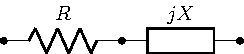
\includegraphics[height=0.1\textheight]{../figs/Z.pdf}
\end{center}
\[
  \overline{U} = \overline{Z} \cdot \overline{I}
\]
\[
  \overline{Z} = R + j X
\]
\end{column}

\begin{column}{0.5\columnwidth}
\begin{center}
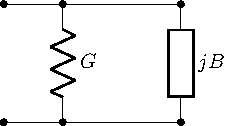
\includegraphics[height=0.25\textheight]{../figs/Y.pdf}
\end{center}
\[
  \overline{I} = \overline{Y} \cdot \overline{U}
\]
\[
  \overline{Y} = G + j B
\]
\end{column}
\end{columns}

\[
\boxed{
  \overline{Y} = \frac{1}{\overline{Z}} \rightarrow \left\{%
    \begin{array}{l}
      |Y| = \frac{1}{|Z|}\\
      \theta_Y = -\theta_Z = -\theta\\
      \end{array}\right.
      }
\]
\end{frame}

\begin{frame}[label={sec:org06eb300}]{Impedancia y Admitancia}
\begin{columns}
\begin{column}{0.5\columnwidth}
\begin{center}
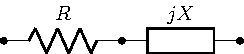
\includegraphics[height=0.1\textheight]{../figs/Z.pdf}
\end{center}

\[
  \overline{Z} = \frac{1}{G + j B} \rightarrow \left\{%
      \begin{array}{l}
	R = \frac{G}{G^2 + B^2}\\
	X = - j \frac{B}{G^2 + B^2}\\
      \end{array}\right.        
\]
\end{column}

\begin{column}{0.5\columnwidth}
\begin{center}
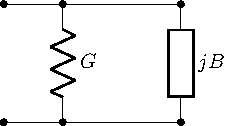
\includegraphics[height=0.25\textheight]{../figs/Y.pdf}
\end{center}

\[
  \overline{Y} = \frac{1}{R + j X} \rightarrow \left\{%
      \begin{array}{l}
	G = \frac{R}{R^2 + X^2}\\
	B = - j \frac{X}{R^2 + X^2}\\
      \end{array}\right.        
\]
\end{column}
\end{columns}
\end{frame}
\section{Potencia}
\label{sec:org2cac24b}
\begin{frame}[label={sec:org629fe43}]{Expresión general}
Sea la tensión referencia de fases. Si \(\theta > 0\) (inductivo) la corriente está retrasada respecto de la tensión (\emph{circuito en retraso}).
\begin{align*}
  u(t) &= U_o \cos \omega t\\
  i(t) &= I_o \cos (\omega t {\color{red}-} \theta)\\
  p(t) &= u(t) \cdot i(t)
\end{align*}
\end{frame}
\begin{frame}[label={sec:org2483d6d}]{Expresión general}
\begin{align*}
  p(t) &= U_o I_o \cdot \cos(\omega t) \cdot \cos(\omega t - \theta) =\\
       &= \frac{1}{2} \cdot U_o I_o \cdot \left(\cos(2\omega t - \theta) + \cos(\theta)\right)\\
       &= U I \cdot \left( \cos(2\omega t - \theta) + \cos(\theta)\right) =\\
       &= U I \cdot \left(\cos(2\omega t)\cos(\theta) + \sin(2\omega t)\sin(\theta) +  \cos(\theta)\right)
\end{align*}

\begin{equation*}
  \boxed{p(t) = U I \cos(\theta) + U I \cos(\theta) \cos(2\omega t) + U I \sin(\theta) \sin(2\omega t)}
\end{equation*}
\end{frame}
\begin{frame}[label={sec:org8bf6bf6}]{Expresión general}
\begin{equation*}
  p(t) = {\color{blue}U I \cos(\theta)} + {\color{blue}U I \cos(\theta)} \cos(2\omega t) + {\color{red}U I \sin(\theta)} \sin(2\omega t)
\end{equation*}

\[
  \color{blue}P = UI\cos\theta \quad%
  \color{red}Q = UI\sin\theta
\]

\begin{equation*}
  \boxed{p(t) = {\color{blue}P} \cdot (1 + \cos(2\omega t)) + {\color{red}Q} \cdot \sin(2\omega t)}
\end{equation*}
\end{frame}


\begin{frame}[label={sec:orga710bec}]{Circuito Resistivo}
   \[
     P = UI\cos\theta \quad%
     {\color{gray}Q = UI\sin\theta}
   \]
   
   \begin{equation*}
p(t) = P \cdot (1 + \cos(2\omega t)) + {\color{gray}Q \cdot \sin(2\omega t)}
\end{equation*}

\noindent\rule{\textwidth}{0.5pt}
\[
  \theta = 0 \rightarrow%
  \left\{% 
    \begin{array}{l}
      P = UI = U^2/R = I^2 R\\
      Q = 0\\
    \end{array}
    \right.
  \]

  \[
    p(t) = P \cdot (1 + \cos(2 \omega t))
  \]
\end{frame}

\begin{frame}[label={sec:org723cd2a}]{Circuito Resistivo}
\begin{center}
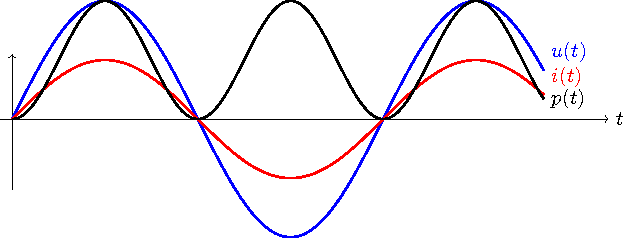
\includegraphics[width=.9\linewidth]{../figs/resistivoPotencia.pdf}
\end{center}

\begin{itemize}
\item Fluctúa al doble de frecuencia.
\item Es siempre positiva.
\end{itemize}
\end{frame}

\begin{frame}[label={sec:org62e37d2}]{Circuito Inductivo puro}
   \[
     {\color{gray}P = UI\cos\theta} \quad%
     Q = UI\sin\theta
   \]
   
   \begin{equation*}
p(t) = {\color{gray}P \cdot (1 + \cos(2\omega t))} + Q \cdot \sin(2\omega t)
\end{equation*}

\noindent\rule{\textwidth}{0.5pt}

\[
  \theta = \pi/2 \rightarrow%
  \left\{% 
    \begin{array}{l}
      P = 0\\
      Q = UI = \frac{U^2}{\omega L} = I^2 \omega L\\
    \end{array}
    \right.
  \]

\[
  p(t) = Q \cdot \sin(2 \omega t)
\]
\end{frame}

\begin{frame}[label={sec:orge8bbe3a}]{Circuito Inductivo puro}
\begin{center}
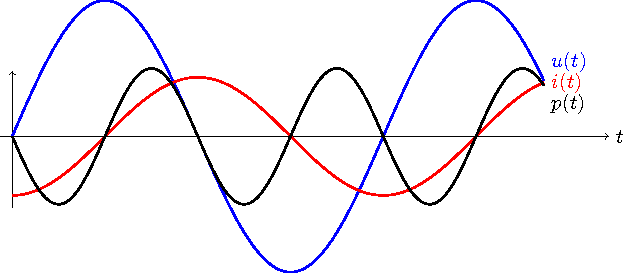
\includegraphics[width=.9\linewidth]{../figs/inductivoPuroPotencia.pdf}
\end{center}

\begin{itemize}
\item Fluctúa al doble de frecuencia.
\item Pasa por los ceros de tensión y corriente.
\item Su valor medio es nulo.
\end{itemize}
\end{frame}

\begin{frame}[label={sec:orgebae9ec}]{Circuito Capacitivo puro}
   \[
     {\color{gray}P = UI\cos\theta} \quad%
     Q = UI\sin\theta
   \]
   
   \begin{equation*}
p(t) = {\color{gray}P \cdot (1 + \cos(2\omega t))} + Q \cdot \sin(2\omega t)
\end{equation*}

\noindent\rule{\textwidth}{0.5pt}

\[
  \theta = -\pi/2 \rightarrow%
  \left\{% 
    \begin{array}{l}
      P = 0\\
      Q = -UI = -U^2 \omega C = - \frac{I^2}{\omega C}\\
    \end{array}
    \right.
  \]
\[
  p(t) = Q \cdot \sin(2 \omega t)
\]
\end{frame}

\begin{frame}[label={sec:orgfe03899}]{Circuito Capacitivo puro}
\begin{center}
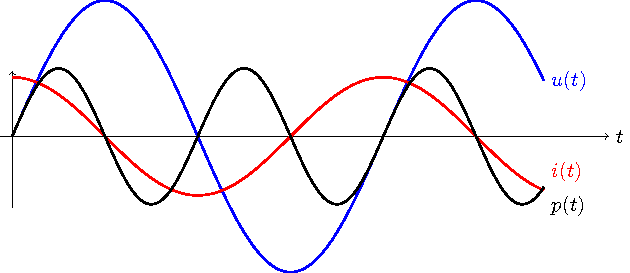
\includegraphics[width=.9\linewidth]{../figs/capacitivoPuroPotencia.pdf}
\end{center}

\begin{itemize}
\item Fluctúa al doble de frecuencia.
\item Pasa por los ceros de tensión y corriente.
\item Su valor medio es nulo.
\end{itemize}
\end{frame}

\begin{frame}[label={sec:org3b51041}]{Circuito Inductivo con pérdidas}
\begin{center}
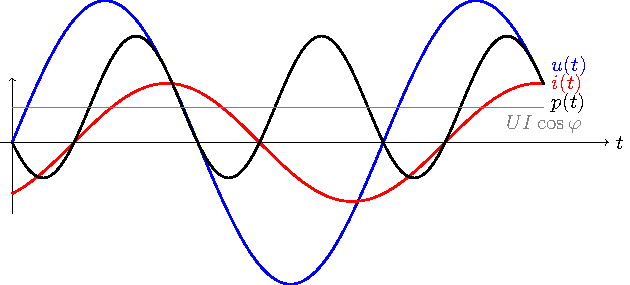
\includegraphics[height=0.5\textheight]{../figs/inductivoPotencia.pdf}
\end{center}

\[
     p(t) = P \cdot (1 + \cos(2\omega t)) + Q \cdot \sin(2\omega t)
\]

\begin{center}
Valor medio positivo, \(P = U I \cos \theta\)
\end{center}
\end{frame}


\begin{frame}[label={sec:org31c2e04}]{Circuito Capacitivo con pérdidas}
\begin{center}
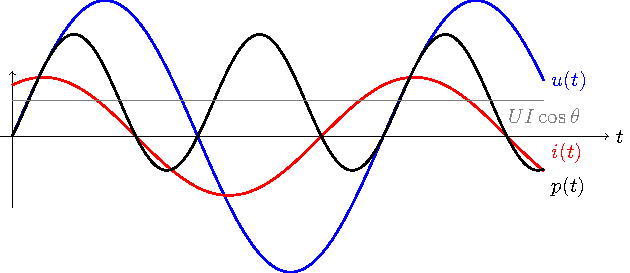
\includegraphics[height=0.5\textheight]{../figs/capacitivoPotencia.pdf}
\end{center}

\[
     p(t) = P \cdot (1 + \cos(2\omega t)) + Q \cdot \sin(2\omega t)
\]

\begin{center}
Valor medio positivo, \(P = U I \cos \theta\)
\end{center}
\end{frame}

\begin{frame}[label={sec:orgd3dc05f}]{Triángulo de Potencias}
\begin{columns}
\begin{column}{0.4\columnwidth}
\begin{itemize}
\item Potencia Activa [\(W\)]
\end{itemize}
\[  
\boxed{P = U\cdot I\cdot\cos(\theta) = R \cdot I^2}
\]

\begin{itemize}
\item Potencia Reactiva [\(VA_r\)]
\end{itemize}
\[
\boxed{Q = U\cdot I\cdot\sin(\theta) = X \cdot I^2}
\]

\begin{itemize}
\item Potencia Aparente [\(VA\)]
\end{itemize}
\[
\boxed{\overline{S} = P + jQ = \overline{U} \cdot \overline{I}^*}
\]

{\footnotesize\begin{align*}
  \overline{U} &= U\phase{0}\\
  \overline{I} &= I\phase{-\theta}\\
                \overline{U} \overline{I}^* &= U\phase{0} \cdot I\phase{\theta} = UI\phase{\theta}\\
                &= U I (\cos\theta + j \sin\theta) = \\
                &= P + j Q
\end{align*}}
\end{column}

\begin{column}{0.6\columnwidth}
\begin{center}
\includegraphics[width=.9\linewidth]{../figs/trianguloPotencias.pdf}
\end{center}

\[
|S| = U \cdot I
\]
\[
\theta_S = \theta_Z = \theta
\]
\[
f.d.p. \equiv \cos(\theta)
\]
\end{column}
\end{columns}
\end{frame}
\begin{frame}[label={sec:org78c88e7}]{Potencia de elementos: Resistencia}
\[
\theta = 0 \Rightarrow 
\begin{cases}
  P_R = R I^2\\
  Q_R = 0\\
  S_R = P_R
\end{cases}
\]

\begin{itemize}
\item Consume potencia activa
\item No consume potencia reactiva
\end{itemize}
\end{frame}

\begin{frame}[label={sec:orga49f968}]{Potencia de elementos: Inductancia}
\[
\theta = \pi/2 \Rightarrow 
\begin{cases}
  P_L = 0\\
  Q_L = \omega L I^2\\
  \overline{S}_L = \omega L I^2 \phase{\pi/2}
\end{cases}
\]

\begin{itemize}
\item No consume potencia activa
\item Consume potencia reactiva (\(Q > 0\))
\end{itemize}
\end{frame}

\begin{frame}[label={sec:orgfc1d2de}]{Potencia de elementos: Condensador}
\[
\theta = - \pi/2 \Rightarrow 
\begin{cases}
  P_L = 0\\
  Q_C = - \omega C U^2\\
  \overline{S}_C = \omega C U^2 \phase{-\pi/2}
\end{cases}
\]

\begin{itemize}
\item No consume potencia activa
\item Genera potencia reactiva (\(Q < 0\))
\end{itemize}
\end{frame}

\begin{frame}[label={sec:org8c97ab6}]{Teorema de Boucherot}
\begin{itemize}
\item En un circuito con múltiples elementos, la potencia aparente total es la suma de las potencias aparentes individuales.
\end{itemize}
\begin{align*}
  \overline{S} &= \sum_{i = 1}^{n} \overline{S}_i\\
  P + jQ &= \sum^n_{i = 1} (P_i + jQ_i)
\end{align*}

\begin{itemize}
\item La potencia activa (reactiva) total es la suma de las potencias activas (reactivas) individuales.
\end{itemize}

\begin{align*}
P &= \sum_{i = 1}^n P_i\\
Q &= \sum_{i = 1}^n Q_i
\end{align*}
\end{frame}

\begin{frame}[label={sec:org139e09e}]{Medida de potencia}
\begin{center}
\includegraphics[height=0.7\textheight]{../figs/vatimetro.pdf}
\end{center}

\alert{Vatímetro}: equipo de medida de 4 terminales (1 par para tensión, 1 par para corriente)
\end{frame}

\begin{frame}[label={sec:orgba48fc5}]{Medida de potencia}
\begin{center}
\includegraphics[height=0.5\textheight]{../figs/vatimetro_Z.pdf}
\end{center}


Habitualmente se emplea con 3 terminales cortocircuitando terminales con *.
\[
  \boxed{W = |V| |I| \cos(\theta_V - \theta_I) = P_Z}
\]
\end{frame}

\section{Compensación de reactiva}
\label{sec:org190512f}

\begin{frame}[label={sec:orgf20cd39}]{Factor de potencia}
El factor de potencia, \(\cos(\theta)\), representa la aportación de potencia activa dentro de la potencia aparente.
\[
P = S \cos \theta
\]

Sean dos sistemas con \alert{misma tensión y potencia activa}, y factores de potencia \(\cos \theta_2 < \cos \theta_1\) (\(Q_2 > Q_1\))

\begin{center}
\includegraphics[height=0.5\textheight]{../figs/Fasores_CompensacionReactiva.pdf}
\end{center}
\end{frame}

\begin{frame}[label={sec:org4a4a2df}]{Potencia Aparente}
\begin{center}
\includegraphics[height=0.5\textheight]{../figs/Fasores_CompensacionReactiva.pdf}
\end{center}


El sistema 2 requiere \alert{mayor potencia aparente} (generador mayor) para alimentar la misma potencia activa.
\[
  \left(\frac{P}{\cos \theta_1} = S_1 \right) < \left( S_2 = \frac{P}{\cos \theta_2}\right) 
\]
\end{frame}

\begin{frame}[label={sec:org346f3e2}]{Sección de Conductores}
\begin{center}
\includegraphics[height=0.5\textheight]{../figs/Fasores_CompensacionReactiva.pdf}
\end{center}

El sistema 2 requiere \alert{mayor sección} de cable para transportar la misma potencia activa.
\[
  \left(\frac{P}{U \cos \theta_1} = I_1 \right) < \left( I_2 = \frac{P}{U \cos \theta_2}\right) 
\]
\end{frame}

\begin{frame}[label={sec:org4404635}]{Generación Local de Reactiva}
\begin{itemize}
\item Comúnmente, el factor de potencia es \alert{inductivo} (máquinas eléctricas
industriales).

\item La red debe suministrar potencia reactiva inductiva (influye en secciones de líneas y tamaños de generadores)

\item Es necesario mejorar \alert{localmente} el factor de potencia. Solución
común: utilizar \alert{bancos de condensadores} como suministradores de
potencia reactiva.
\end{itemize}
\end{frame}

\begin{frame}[label={sec:orgfc3dc4f}]{Compensación de Reactiva con Condensadores}
Sea una carga de potencia activa \(P_z\), potencia reactiva \(Q_z\), factor de potencia \(\cos\theta\). Se desea \alert{mejorar el factor de potencia} a \(\cos \theta' > \cos \theta\).

\begin{center}
\includegraphics[height=0.4\textheight]{../figs/Circuito_CompensacionReactiva.pdf}
\end{center}

\begin{align*}
  P' &= P_z\\
  Q' &= Q_c + Q_z \quad (Q' < Q_z)\\
  \overline{I}' &= \overline{I}_c + \overline{I_z} \quad (I' < I_z)\\
\end{align*}
\end{frame}

\begin{frame}[label={sec:org9124dc0}]{Cálculo de la Capacidad}
\begin{center}
\includegraphics[height=0.3\textheight]{../figs/Circuito_CompensacionReactiva.pdf}
\end{center}

\begin{align*}
Q_z &= P_z \tan \theta\\
Q'&= P_z \tan \theta'\\
|Q_c| &= Q_z - Q' = P_z (\tan \theta - \tan \theta')
\end{align*}
\[
|Q_c| = \omega C U^2 \rightarrow \boxed{C = \frac{P_z (\tan \theta - \tan \theta')}{\omega U^2}}
\]
\end{frame}




\section{Teoremas}
\label{sec:orgf8e3645}
\begin{frame}[label={sec:org1c871b9}]{Equivalencia de fuentes}
Sólo es posible establecer equivalencia entre \alert{fuentes reales}.
\begin{columns}
\begin{column}{0.33\columnwidth}
\begin{center}
\includegraphics[height=0.5\textheight]{../figs/FuenteTensionReal.pdf}
\end{center}
\[
  \overline{U}_{AB} = \overline{\epsilon}_g - \overline{Z}_{\epsilon_g} \cdot \overline{I}
\]
\end{column}
\begin{column}{0.33\columnwidth}
\begin{align*}
  \overline{Z}_g &= \overline{Z}_{\epsilon_g} = \overline{Z}_{I_g}\\
  \overline{\epsilon}_g &= \overline{Z}_g \cdot \overline{I}_g\\
  \overline{I}_g &= \frac{\overline{\epsilon}_g}{\overline{Z}_g}
\end{align*}
\end{column}
\begin{column}{0.33\columnwidth}
\begin{center}
\includegraphics[height=0.5\textheight]{../figs/FuenteCorrienteReal.pdf}
\end{center}
\[
  \overline{I} = \overline{I}_g - \frac{\overline{U}_{AB}}{\overline{Z}_{I_g}}
\]
\end{column}
\end{columns}
\end{frame}


\begin{frame}[label={sec:org6ffc400}]{Teorema de superposición}
\begin{columns}
\begin{column}{0.5\columnwidth}
La respuesta de un \alert{circuito lineal} a varias fuentes de excitación actuando simultáneamente es igual a la suma de las respuestas que se tendrían cuando actuase cada una de ellas por separado

\[
y(t) = \sum_i y_i(t)
\]
\end{column}

\begin{column}{0.5\columnwidth}
\begin{center}
\includegraphics[width=.9\linewidth]{../figs/superposicion.pdf}
\end{center}
\end{column}
\end{columns}
\end{frame}

\begin{frame}[label={sec:org6a5142a}]{Teorema de superposición}
\framesubtitle{Análisis de un circuito mediante superposición}
\begin{block}{Procedimiento}
\begin{enumerate}
\item Se apagan todas las fuentes \alert{independientes} del circuito menos una.
\begin{itemize}
\item Las fuentes de tensión se sustituyen por un cortocircuito (\(U = 0\)).
\item Las fuentes de corriente se sustituyen por un circuito abierto (\(I = 0\)).
\item Las fuentes \alert{dependientes} \alert{no} se modifican.
\end{itemize}
\item Se analiza el circuito, obteniendo la respuesta individual a la fuente que permanece activa.
\item Se repite este procedimiento para cada una de las fuentes \alert{independientes} del circuito.
\item La respuesta total del circuito es la suma de las respuestas individuales.
\end{enumerate}
\end{block}
\end{frame}

\begin{frame}[label={sec:orga5f37d4}]{Teorema de superposición}
\framesubtitle{Análisis de un circuito mediante superposición}

\begin{block}{Observaciones}
\begin{itemize}
\item \alert{Siempre} hay que aplicar este método cuando en un circuito conviven fuentes de \alert{diferente frecuencia} (o fuentes de corriente continua y corriente alterna).
\item En el caso de fuentes de corriente alterna \alert{sinusoidal}, la respuesta debe expresarse en el \alert{dominio del tiempo}. \alert{No} se pueden \alert{sumar} los \alert{fasores} que corresponden a \alert{frecuencias diferentes}.
\item En el primer paso del procedimiento, se pueden agrupar las fuentes que funcionan a la misma frecuencia y calcular la respuesta del circuito en esa frecuencia.
\end{itemize}
\end{block}
\end{frame}

\begin{frame}[label={sec:orgee8ab4c}]{Teorema de superposición}
\framesubtitle{Potencia}

El principio de superposición aplica a tensiones y corrientes, pero \alert{no} a potencias. Supongamos \(i(t) = i_1(t) + i_2(t)\):
\begin{align*}
  p(t) &= R \cdot i^2(t) =\\
       &= R \cdot (i_1(t) + i_2(t))^2 =\\
       &=R \cdot (i_1^2(t) + i_2^2(t) + 2\cdot i_1(t) \cdot i_2(t))\\
  p(t) &\neq p_1(t) + p_2(t)
\end{align*}
\end{frame}
\begin{frame}[label={sec:org80aa651}]{Teorema de superposición}
\framesubtitle{Potencia}
\begin{itemize}
\item Cuando las señales son \alert{ortogonales en un período}\footnote{Dos señales son ortogonales si cumplen la siguiente ecuación: \[<f_1, f_2>_T = \int_T f_1(t) \cdot f_2(t) dt = 0\]} se pueden sumar las potencias \alert{medias} de cada circuito.
\end{itemize}
\begin{align*}
  P = \sum_i P_i
\end{align*}
\begin{itemize}
\item Ejemplos de señales ortogonales: sinusoidales con diferente frecuencia, una sinusoide con una continua, \ldots{}
\end{itemize}
\end{frame}

\begin{frame}[label={sec:orge359509}]{Teoremas de Thévenin/Norton}
\framesubtitle{Thévenin}

Cualquier \alert{red lineal} compuesta por elementos activos y pasivos puede sustituirse, desde el punto de vista de sus terminales externos AB, por una \alert{fuente de tensión} (generador de Thévenin, \(\epsilon_{th}\)) en \alert{serie} con una impedancia (impedancia de Thévenin, \(Z_{th}\)).

\begin{center}
\includegraphics[height=0.6\textheight]{../figs/EquivalenteThevenin.pdf}
\end{center}
\end{frame}

\begin{frame}[label={sec:orgca38193}]{Teoremas de Thévenin/Norton}
\framesubtitle{Norton}
Cualquier \alert{red lineal} compuesta por elementos activos y pasivos puede sustituirse, desde el punto de vista de sus terminales externos AB, por una \alert{fuente de corriente} (generador de Norton, \(I_N\)) en \alert{paralelo} con una impedancia (impedancia de Norton, \(Z_N\)).

\begin{center}
\includegraphics[height=0.6\textheight]{../figs/EquivalenteNorton.pdf}
\end{center}
\end{frame}

\begin{frame}[label={sec:org5929b87}]{Teoremas de Thévenin/Norton}
\framesubtitle{Cálculo del equivalente de Thévenin}
\begin{center}
\includegraphics[height=0.38\textheight]{../figs/EquivalenteThevenin.pdf}
\end{center}

\begin{itemize}
\item Circuito Abierto (\(Z_L \to \infty, \quad U_{AB} = U_{oc}\))
\end{itemize}
\[
\boxed{\epsilon_{th} = U_{oc}}
\]
\begin{itemize}
\item Cortocircuito (\(Z_L = 0, \quad I = I_{sc}\))
\end{itemize}
\[
\boxed{Z_{th} = \frac{\epsilon_{th}}{I_{sc}} = \frac{U_{oc}}{I_{sc}}}
\]
\end{frame}

\begin{frame}[label={sec:orgc83c1ac}]{Teoremas de Thévenin/Norton}
\framesubtitle{Cálculo del equivalente de Norton}
\begin{center}
\includegraphics[height=0.38\textheight]{../figs/EquivalenteNorton.pdf}
\end{center}

\begin{itemize}
\item Cortocircuito (\(Z_L = 0, \quad I = I_{sc}\))
\end{itemize}
\[
\boxed{I_N = I_{sc}}
\]
\begin{itemize}
\item Circuito Abierto (\(Z_L \to \infty, \quad U_{AB} = U_{oc}\))
\end{itemize}
\[
\boxed{Z_N = \frac{U_{oc}}{I_N} = \frac{U_{oc}}{I_{sc}}}
\]
\end{frame}

\begin{frame}[label={sec:org44f2a31}]{Teoremas de Thévenin/Norton}
\framesubtitle{Cálculo de Thévenin/Norton}

\begin{block}{Observaciones}
\begin{itemize}
\item Cálculo de la impedancia:
\begin{itemize}
\item Si el circuito \alert{no} contiene fuentes dependientes, se puede realizar \alert{apagando} todos los \alert{generadores} y obteniendo la impedancia equivalente.
\item Si el circuito contiene fuentes dependientes, es necesario conectar un \alert{generador de prueba} a la salida del circuito y obtener la relación entre la tensión y corriente de este generador.
\end{itemize}

\item Gracias a la equivalencia de fuentes, una vez obtenido uno de los equivalentes se puede obtener el otro mediante una transformación.
\end{itemize}
\end{block}
\end{frame}

\begin{frame}[label={sec:org6d7d50e}]{Máxima Transferencia de Potencia}
\framesubtitle{Planteamiento}
Sea el circuito lineal de la figura. ¿Qué impedancia \(Z_L\) hay que conectar en los terminales AB para que el circuito entregue la máxima potencia disponible?

\begin{center}
\includegraphics[height=0.55\textheight]{../figs/EquivalenteThevenin.pdf}
\end{center}

Resolvemos esta pregunta mediante el generador equivalente de Thévenin.
\end{frame}



\begin{frame}[label={sec:org7accf87}]{Máxima Transferencia de Potencia}
\framesubtitle{Ecuaciones}
Calculamos la potencia activa en la impedancia de carga \(Z_L\):
\begin{columns}
\begin{column}{0.3\columnwidth}
\begin{center}
\includegraphics[height=0.45\textheight]{../figs/EquivalenteThevenin0.pdf}
\end{center}
\end{column}

\begin{column}{0.2\columnwidth}
\begin{align*}
  \overline{Z}_{th} &= R_{th} + jX_{th}\\
  \overline{Z}_L &= R_L + jX_L\\
\end{align*}
\end{column}

\begin{column}{0.4\columnwidth}
\begin{align*}
\overline{I} &= \frac{\overline{\epsilon}_{th}}{\overline{Z}_{th} + \overline{Z}_L}\\
P_L &= I^2 \cdot R_L\\
\Aboxed{P_L &= \frac{\epsilon^2_{th}}{|\overline{Z}_{th} + \overline{Z}_L|^2} \cdot R_L}
\end{align*}
\end{column}
\end{columns}

Las condiciones de máximo son: 
\[
  \boxed{%
    \diffp{P_L}{X_L} = 0 \quad%
    \diffp{P_L}{R_L} = 0%
  }
\]
\end{frame}

\begin{frame}[label={sec:orged8e53e}]{Máxima Transferencia de Potencia}
\framesubtitle{Reactancia}
A partir de la expresión de potencia en la carga\ldots{}
\[
  P_L = \frac{\epsilon^2_{th}}{|\overline{Z}_{th} + \overline{Z}_L|^2} \cdot R_L
\]
calculamos la derivada parcial respecto de la reactancia:
\[
  \diffp{P_L}{X_L} = \epsilon^2_{th} \cdot R_L \cdot \left[\frac{-1}{\left((R_L + R_{th})^2 + (X_L + X_{th})^2\right)^2} \cdot 2 \cdot (X_L + X_{th})\right]
\]
Aplicamos la condición de máximo y obtenemos un resultado parcial:
\[
   \diffp{P_L}{X_L} = 0 \Rightarrow \boxed{X_L = - X_{th}}
\]
\end{frame}

\begin{frame}[label={sec:org48aca49}]{Máxima Transferencia de Potencia}
\framesubtitle{Resistencia}
Simplificamos la expresión de la potencia teniendo en cuenta el resultado anterior (\(X_L = - X_{th}\)):
\[
  P_L = \frac{\epsilon^2_{th}}{(R_{th} + R_L)^2} \cdot R_L
\]
Calculamos la derivada parcial respecto de la resistencia:
\begin{align*}
  \diffp{P_L}{R_L} &= \epsilon^2_{th} \cdot \left[\frac{1}{(R_L + R_{th})^2} - 2 \cdot \frac{R_L}{(R_L + R_{th})^3}\right]\\
		   &= \frac{\epsilon^2_{th} \cdot (R_{th} - R_L)}{(R_L + R_{th})^3}
\end{align*}
Nuevamente, aplicamos la condición de máximo y obtenemos la resistencia:
\[
   \diffp{P_L}{R_L} = 0 \Rightarrow \boxed{R_L = R_{th}}
\]
\end{frame}

\begin{frame}[label={sec:org98f2503}]{Máxima Transferencia de Potencia}
\framesubtitle{Impedancia de carga}

Dado un circuito lineal (del que podemos calcular su equivalente de Thévenin) \ldots{}
\begin{center}
\includegraphics[height=0.45\textheight]{../figs/EquivalenteThevenin.pdf}
\end{center}

\ldots{} la impedancia de carga que hay que conectar entre sus terminales AB para obtener la máxima potencia disponible es:
\[
  \boxed{\overline{Z}_L = \overline{Z}_{th}^*}
\]
\end{frame}

\begin{frame}[label={sec:orgcef1d7f}]{Máxima Transferencia de Potencia}
\framesubtitle{Máxima potencia disponible}

La máxima potencia disponible en la carga es:
\begin{center}
\includegraphics[height=0.45\textheight]{../figs/EquivalenteThevenin.pdf}
\end{center}

\begin{equation*}
  \left.
    \begin{matrix}
      \overline{Z}_L = \overline{Z}_{th}^*\\
      P_L = \frac{\epsilon^2_{th}}{|\overline{Z}_{th} + \overline{Z}_L|^2} \cdot R_L
    \end{matrix} \right\}\rightarrow
  \boxed{P_L = \frac{\epsilon^2_{th}}{4 R_{th}}}
\end{equation*}
\end{frame}
\end{document}